\documentclass[hyperref={pdfpagelabels=false},aspectratio=34,14pt]{beamer}
\usepackage{lmodern} %TODO: descobrir o que mudou as fontes dos slides (comparar com os primeiros)
\usepackage[utf8]{inputenc}
\usepackage[T1]{fontenc}
\usefonttheme[onlymath]{serif}
\usepackage[brazil]{babel}
\usepackage[outputdir=..]{minted}
\usepackage{xcolor}
\usepackage{soul} % strikethrough
\usepackage{advdate}
\usepackage{graphicx}
\usepackage[ampersand]{easylist}
\usepackage{multirow}
\usepackage{tikz}
\usetikzlibrary{shapes,arrows,positioning}
\usetikzlibrary{circuits.logic.US}
\usetikzlibrary{matrix,calc}
\usepackage{karnaugh-map}

\usepackage{pgfpages}
\setbeamertemplate{note page}{\pagecolor{yellow!5}\insertnote}\usepackage{palatino}
\newcommand{\yes}{edge node [above] {yes}}
\newcommand{\no}{edge  node [left]  {no}}
\newcommand{\textttb}[1]{\textcolor{blue}{\ttfamily #1}}

% \setmathfont{Latin Modern Math}[version=lm]

\graphicspath{{../figs/}}

\definecolor{bgc}{rgb}{0.95,0.9,0.95}
\definecolor{links}{HTML}{2A7F7F}
\hypersetup{colorlinks,linkcolor=,urlcolor=links}

\newminted{verilog}{fontsize=\scriptsize, 
		   linenos,
		   numbersep=8pt,
           bgcolor=bgc,
           tabsize=4,
		   framesep=3mm} 
%		   frame=lines,

\newcommand{\verilog}[1]{\verilogf{#1}{\footnotesize}

\newcommand{\verilogf}[2]{\inputminted[fontsize=#2, 
		   linenos,
		   tabsize=2,
		   numbersep=4pt,
           bgcolor=bgc,
		   framesep=3mm]{verilog}{../codes/#1.v}
}

\newminted{nasm}{fontsize=\scriptsize, 
		   linenos,
		   numbersep=8pt,
           bgcolor=bgc,
		   framesep=3mm} 

% \author[shortname]{\scriptsize Prof. Edilson Kato \and Prof. Maurício Figueiredo \and Prof. Ricardo Menotti\newline
% \href{mailto:kato@ufscar.br}{kato@ufscar.br} \and    \href{mailto:mauricio@ufscar.br}{mauricio@ufscar.br} \and
% \href{mailto:menotti@ufscar.br}{menotti@ufscar.br}}

\newcommand{\newauthor}[2]{
  \parbox{0.40\textwidth}{
    \texorpdfstring
      {
        \centering
        \footnotesize #1 \newline
        {\scriptsize{\urlstyle{same}\href{mailto:#2}{#2}\urlstyle{tt}}}
      }
      {#1} \newline
  }
}

\author{
%   \newauthor{Prof. Edilson Kato}{kato@ufscar.br}
% \and
  \newauthor{Prof. Ricardo Menotti}{menotti@ufscar.br}
\and 
  \newauthor{Prof. Maurício Figueiredo}{mauricio@ufscar.br}
% \and
%   \newauthor{Prof. Roberto Inoue}{rsinoue@ufscar.br}
}

\institute{\href{http://www.dc.ufscar.br/}{Departamento de Computação} \\
           \href{http://www.ufscar.br/}{Universidade Federal de São Carlos}} 
\titlegraphic{
  \makebox[.85\paperwidth]{
    
\includegraphics[height=1cm]{figs/LogoDC} 
    \hfill 
    
\includegraphics[height=1cm]{figs/LogoUfscar}}}
\date{Atualizado em: \today} 
% \date{\DayAfter[+1]} % +/-

%\logo{
\includegraphics[height=1cm]{figs/LogoUfscar}
\includegraphics[height=1cm]{figs/LogoDC}}

\title{Lógica Digital (1001351)}

\AtBeginSubsection[]
{
  \begin{frame}<beamer>{Roteiro}
    \tableofcontents[currentsection,currentsubsection]
  \end{frame}
}

\addtobeamertemplate{navigation symbols}{}{%
    \usebeamerfont{footline}%
    \usebeamercolor[fg]{footline}%
    \hspace{1em}%
    \raisebox{1.2pt}[0pt][0pt]{\insertframenumber/\inserttotalframenumber}
}


\title{Unidade Lógica e Aritmética}

\subtitle{Laboratório de Arquitetura e Organização de Computadores I} % prática

\begin{document}

\begin{frame}
	\titlepage
\end{frame} 

% \begin{frame}{Roteiro}
%   \tableofcontents
%   % You might wish to add the option [pausesections]
% \end{frame}

% Section and subsections will appear in the presentation overview
% and table of contents.

\section{Unidade Lógica e Aritmética}

\subsection{Conceitos} 

\frame{
    \frametitle{Operations}
    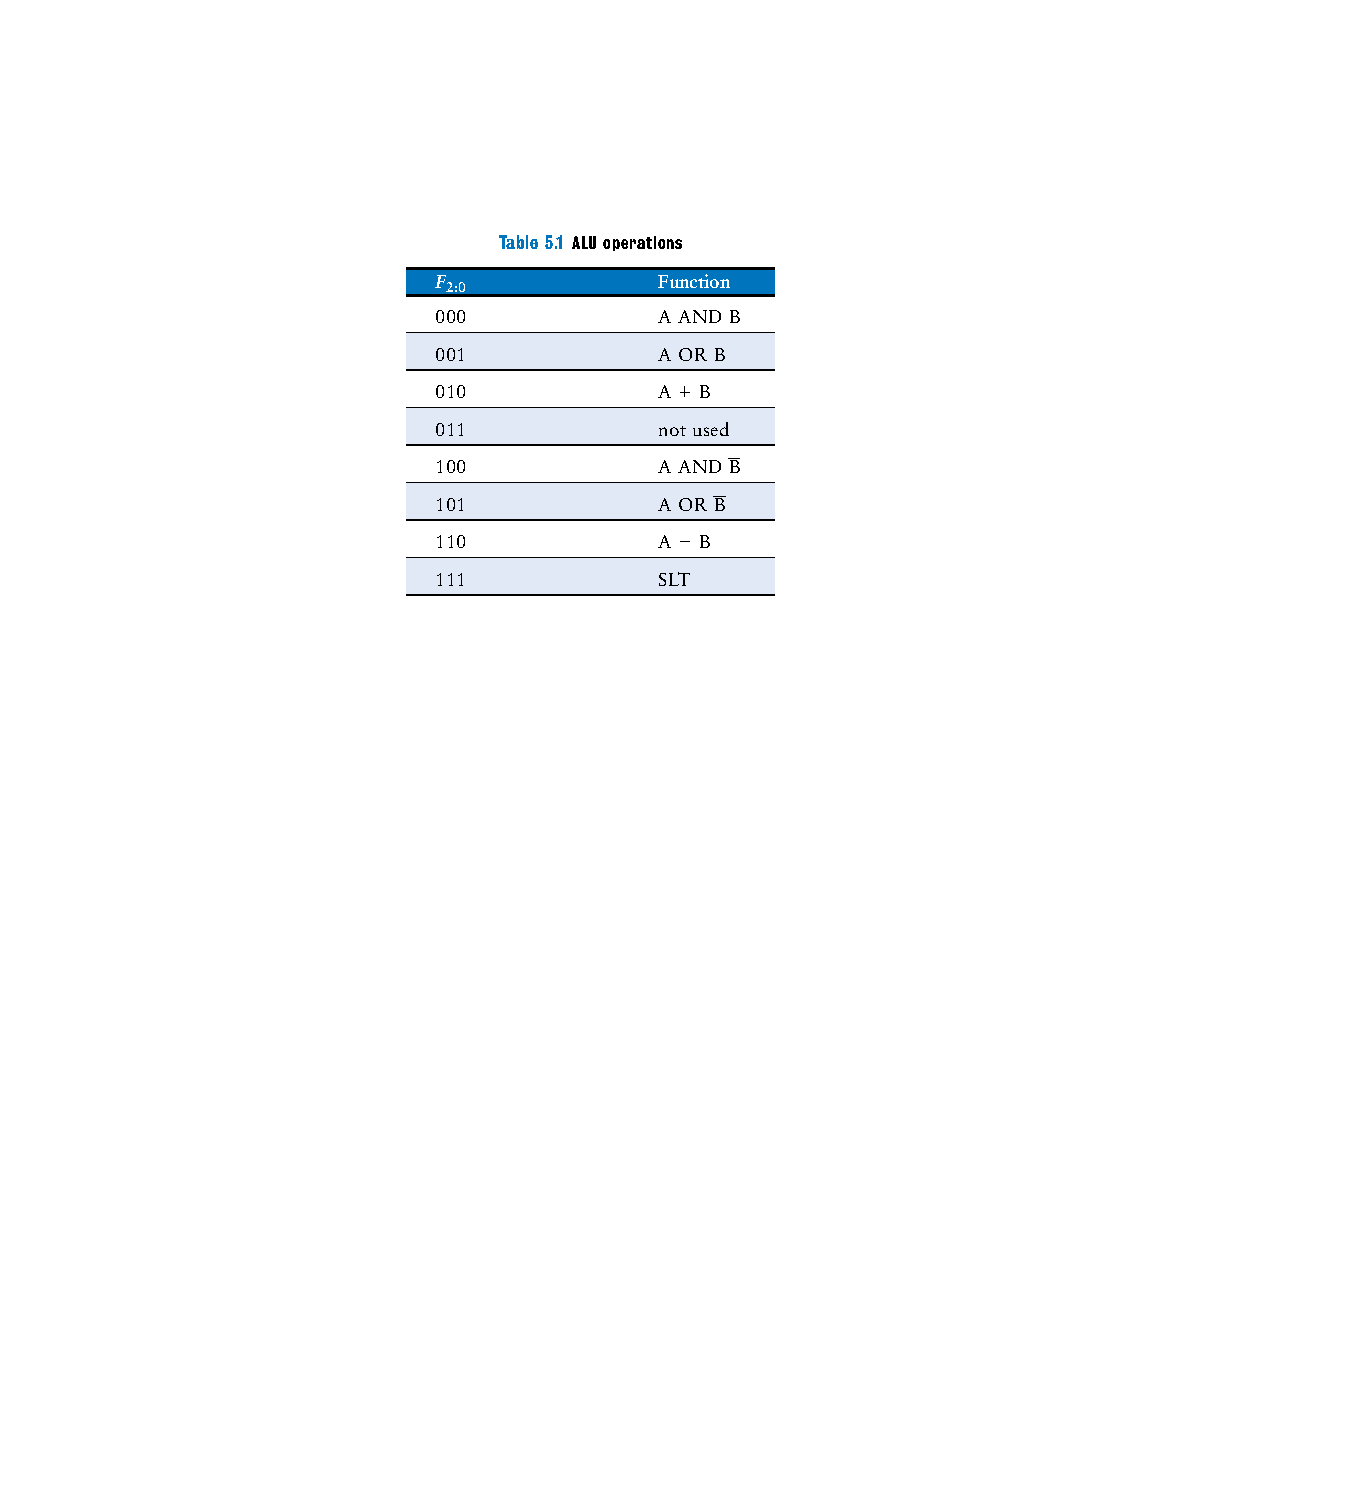
\includegraphics[scale=.7]{figs/aluop}
}

\frame{
    \frametitle{Esquemático}
    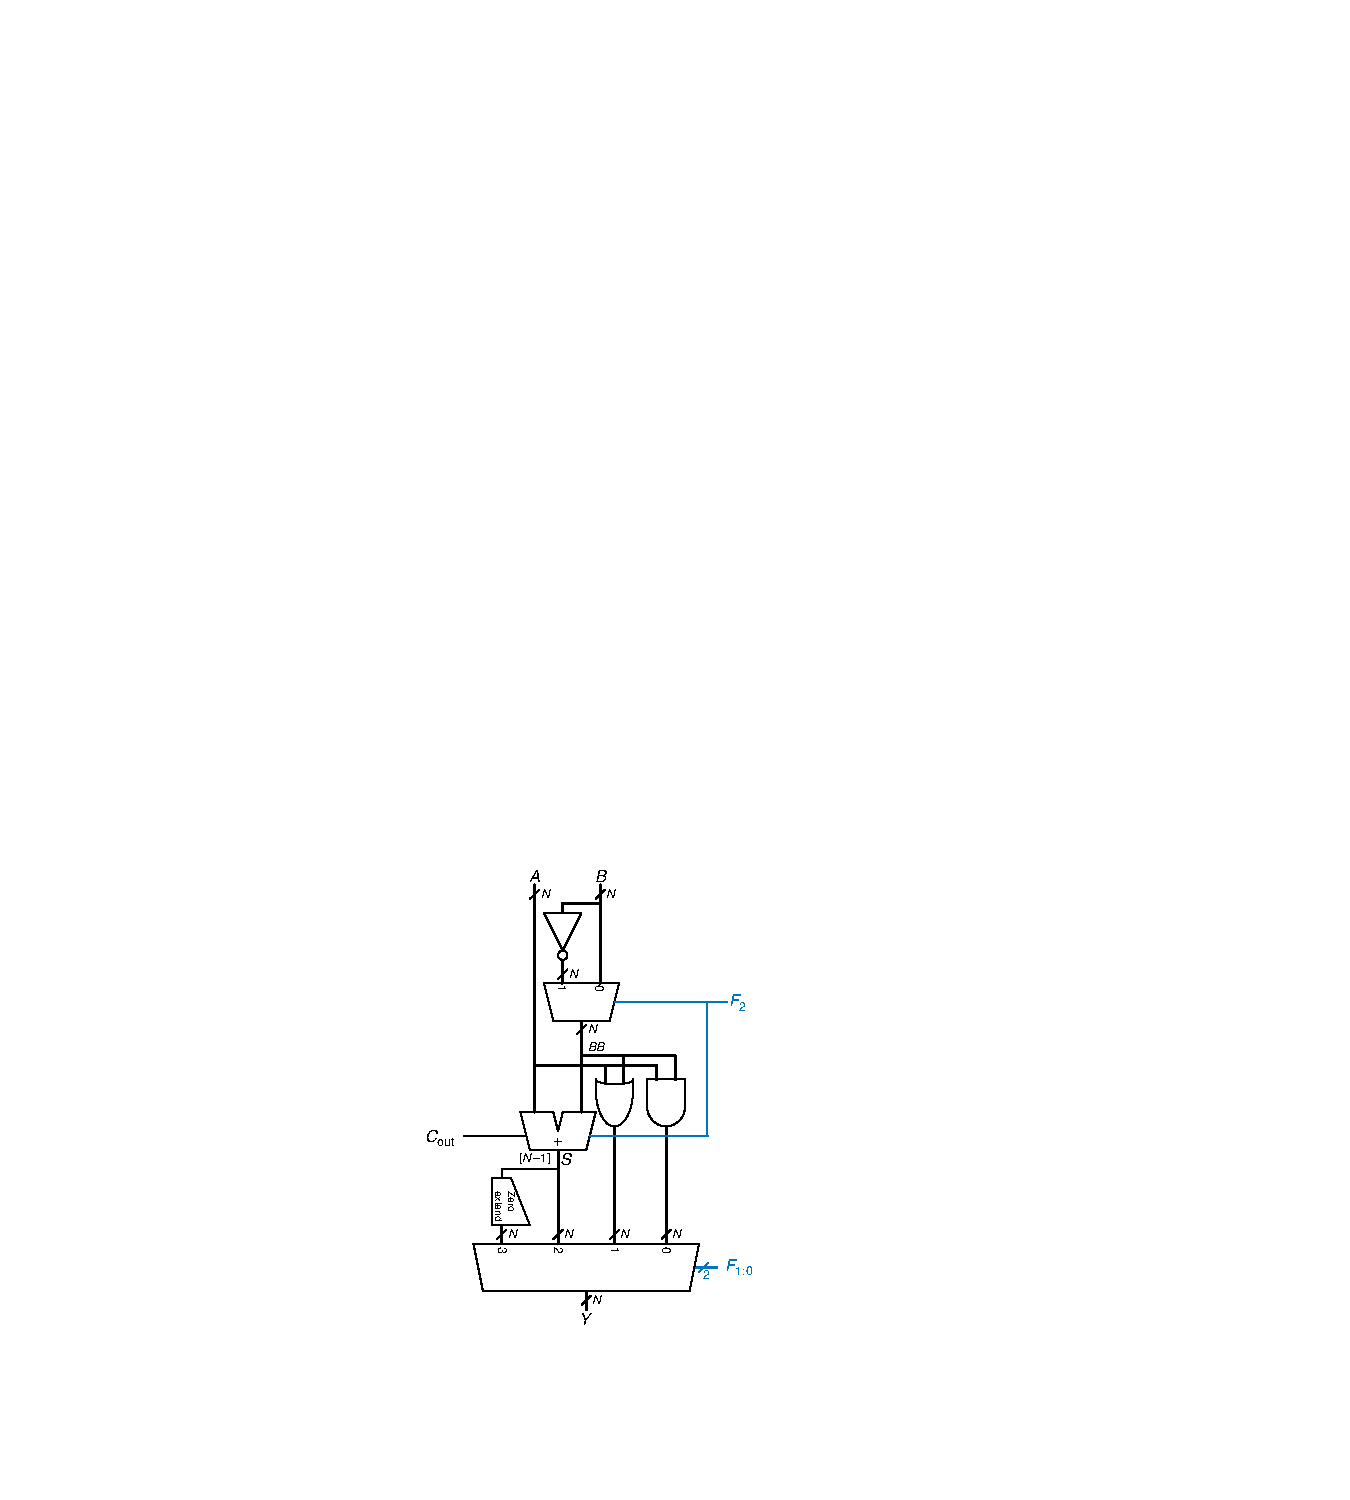
\includegraphics[scale=.7]{figs/aluschem}
}

\subsection{Implementação (I)} 

\begin{frame}[fragile]
	\frametitle{Unidade Lógica e Aritmética}
	\begin{verilogcode}
module alu(input  logic [31:0] a, b,
           input  logic [ 2:0]  f,
           output logic [31:0] y,
           output logic zero);
           
  logic [31:0] bb, b2, add_res, and_res, or_res, slt_res;
  
  assign bb = ~b;
  assign b2 = f[2] ? bb : b;
  assign add_res = a + b2 + f[2]; // handle 2's complement
  assign and_res = a & b2;
  assign or_res  = a | b2;
  assign slt_res = add_res[31] ? 32'b1 : 32'b0;
  
  always_comb
    case (f[1:0])
      2'b00: y = and_res;
      2'b01: y = or_res;
      2'b10: y = add_res;
      2'b11: y = slt_res;
    endcase
    
  assign zero = (y == 32'b0);
endmodule
    \end{verilogcode} 
\end{frame}


\begin{frame}[fragile]
	\frametitle{Test bench}
	\begin{verilogcode}
module talu();
  logic clk;
  logic [31:0] a, b, y, y_expected;
  logic [ 2:0] f;
  logic        zero, zero_expected;

  logic [31:0] vectornum, errors;
  logic [103:0] testvectors[10000:0];

  alu dut(a, b, f, y, zero);

  always begin
    clk = 1; #50; clk = 0; #50;
  end

  initial begin
    $readmemh("talu.tv", testvectors);
    vectornum = 0; errors = 0;
  end
    \end{verilogcode} 
\end{frame}

\begin{frame}[fragile]
	\frametitle{Test bench}
	\begin{verilogcode}
  always @(posedge clk)
    begin
      #1; 
      f = testvectors[vectornum][102:100];
      a = testvectors[vectornum][99:68];
      b = testvectors[vectornum][67:36];
      y_expected = testvectors[vectornum][35:4];
      zero_expected = testvectors[vectornum][0];
    end

 always @(negedge clk) 
   begin
     if (y !== y_expected || zero !== zero_expected) begin
       $display("Error in vector %d", vectornum);
       $display(" Inputs : a = %h, b = %h, f = %b", a, b, f);
       $display(" Outputs: y = %h (%h expected), zero = %h (%h expected)", 
         y, y_expected, zero, zero_expected); 
       errors = errors+1;
     end
     vectornum = vectornum + 1;
     if (testvectors[vectornum][0] === 1'bx) begin
       $display("%d tests completed with %d errors", vectornum, errors);
       $stop;
     end
   end
endmodule
    \end{verilogcode} 
\end{frame}

\begin{frame}[fragile]
	\frametitle{Test vectors}
	\begin{verilogcode}
2_00000000_00000000_00000000_1
2_00000000_FFFFFFFF_FFFFFFFF_0
2_00000001_FFFFFFFF_00000000_1
2_000000FF_00000001_00000100_0
6_00000000_00000000_00000000_1
6_00000000_FFFFFFFF_00000001_0
6_00000001_00000001_00000000_1
6_00000100_00000001_000000FF_0
7_00000000_00000000_00000000_1
7_00000000_00000001_00000001_0
7_00000000_FFFFFFFF_00000000_1
7_00000001_00000000_00000000_1
7_FFFFFFFF_00000000_00000001_0
0_FFFFFFFF_FFFFFFFF_FFFFFFFF_0
0_FFFFFFFF_12345678_12345678_0
0_12345678_87654321_02244220_0
0_00000000_FFFFFFFF_00000000_1
1_FFFFFFFF_FFFFFFFF_FFFFFFFF_0
1_12345678_87654321_97755779_0
1_00000000_FFFFFFFF_FFFFFFFF_0
1_00000000_00000000_00000000_1
    \end{verilogcode} 
\end{frame}


\begin{frame}
	\titlepage
\end{frame} 

\end{document}
